\documentclass[border=3pt]{standalone}
% Preâmbulo compartilhado pelos diagramas TikZ da aula 5 de IHC (Processos de Design)
\usepackage[T1]{fontenc}
\usepackage[utf8]{inputenc}
\usepackage{lmodern}
\usepackage{amsmath}
\usepackage{xcolor}
\usepackage{tikz}
\usetikzlibrary{arrows.meta,angles,quotes,decorations.pathmorphing,calc,
                positioning,shapes.geometric,shapes.misc,backgrounds,fit,
                math}

% Paleta (mesma dos SVGs originais)
% Paleta da disciplina de IHC: acento roxo (#755099), da capa do livro.
% (o nome "dblue" é mantido para não alterar todos os diagramas)
\definecolor{dblue}{HTML}{755099}
\definecolor{dorange}{HTML}{B3541E}
\definecolor{dgreen}{HTML}{4A7C59}
\definecolor{dred}{HTML}{9C4B4B}
\definecolor{dcream}{HTML}{F4F1EA}
\definecolor{dshade}{HTML}{DDD7C9}

% Função gaussiana (não normalizada por padrão de escala visual)
\pgfmathdeclarefunction{gauss}{3}{%
  \pgfmathparse{1/(#3*sqrt(2*pi))*exp(-((#1-#2)^2)/(2*#3^2))}%
}

% Estilos comuns (prefixo d... para não colidir com chaves internas do pgf)
\tikzset{
  >={Stealth[length=2mm]},
  dguide/.style={gray!55, dashed, line width=0.4pt},
  daxis/.style={gray!60, line width=0.7pt, ->},
  dbody/.style={fill=black!3, draw=black!80, line width=1pt},
  dacc/.style={draw=dblue, line width=1pt},
  dlbl/.style={black!55, font=\small},
  dsub/.style={black!45, font=\footnotesize},
  dstate/.style={circle, draw=black!80, fill=dcream, line width=1pt,
                 minimum size=17mm, font=\large, inner sep=1pt},
  dobs/.style={circle, draw=black!80, fill=dshade, line width=1pt,
               minimum size=14mm, font=\large, inner sep=1pt},
  dbox/.style={rounded corners=2pt, draw=black!80, fill=dcream, line width=1pt,
               align=center, inner sep=6pt},
  dop/.style={circle, draw=black!80, fill=white, line width=1pt,
              minimum size=6mm, inner sep=0pt, font=\small},
  dtrans/.style={->, dblue, line width=1pt},
  dmeas/.style={->, dorange, line width=1pt},
  dcurve/.style={line width=1pt, dblue},
  dcurveb/.style={line width=1.4pt, dorange},
}

\begin{document}
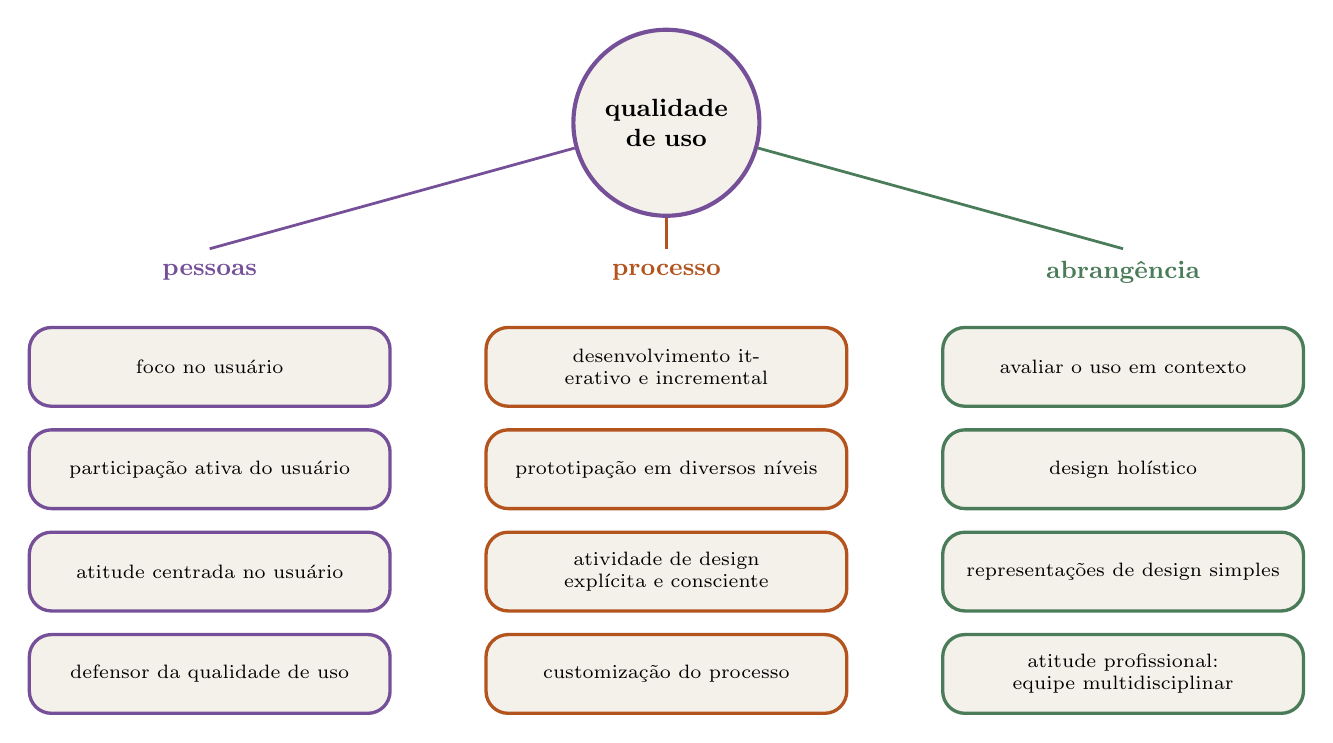
\begin{tikzpicture}[x=1cm,y=1cm,
   p/.style={dbox, rounded corners=8pt, text width=4.3cm, minimum height=1.0cm, font=\scriptsize, inner sep=4pt}]

  \node[dstate, minimum size=22mm, font=\small, text width=2.2cm, align=center, draw=dblue, line width=1.5pt] (h) at (7.4,5.1) {\textbf{qualidade de uso}};

  \node[font=\small\bfseries, dblue] at (1.6,3.2) {pessoas};
  \node[font=\small\bfseries, dorange] at (7.4,3.2) {processo};
  \node[font=\small\bfseries, dgreen] at (13.2,3.2) {abrangência};

  \foreach \y/\t in {2.0/{foco no usuário},0.7/{participação ativa do usuário},-0.6/{atitude centrada no usuário},-1.9/{defensor da qualidade de uso}} { \node[p, draw=dblue, line width=1.2pt] at (1.6,\y) {\t}; }
  \foreach \y/\t in {2.0/{desenvolvimento iterativo e incremental},0.7/{prototipação em diversos níveis},-0.6/{atividade de design explícita e consciente},-1.9/{customização do processo}} { \node[p, draw=dorange, line width=1.2pt] at (7.4,\y) {\t}; }
  \foreach \y/\t in {2.0/{avaliar o uso em contexto},0.7/{design holístico},-0.6/{representações de design simples},-1.9/{atitude profissional: equipe multidisciplinar}} { \node[p, draw=dgreen, line width=1.2pt] at (13.2,\y) {\t}; }

  \draw[dblue, line width=1pt] (h) -- (1.6,3.5); \draw[dorange, line width=1pt] (h) -- (7.4,3.5); \draw[dgreen, line width=1pt] (h) -- (13.2,3.5);

\end{tikzpicture}
\end{document}
